\section{Traditional Approaches to Graph Learning}
\subsection{Node-level statistics}
Prior to advent of deep learning on graphs, a large part of machine learning on graphs was directed towards extraction of statistics/features based on heuristic functions and domain knowledge from graphs, and passing this information to a machine learning classifier. Now, we look over common node-level statistics.
\begin{definition}[Node degree]
The degree $d_u$ of a node $u \in V$ is the number of edges incident to a node, and in terms of $\mathbf{A}$ for a simple graph
\begin{equation} \label{eq:degree}
	d_u = \sum_{v \in V} A_{uv}
\end{equation}
If our graph is directed or weighted, we can have the notion of in-degree and out-degree by summing over rows or columns in Equation (\ref{eq:degree}).
\end{definition}
\marginnote{\textit{Perron-Frobenius Theorem}: A real square matrix with positive entries has a unique largest real eigenvalue, and the corresponding eigenvector can be chosen to have strictly positive components.}
\begin{definition}[Eigenvector Centrality]
The eigenvector centrality $e_u$ of a node $u \in V$ is defined by the recurrence relation
\begin{equation}
	e_u = \dfrac{1}{\lambda} \sum_{v\in V} A_{uv}e_v \; \forall \; u \in V
\end{equation}	
We can rewrite the above equation to notice that $\mathbf{A}\mathbf{e} = \lambda \mathbf{e}$ where $\mathbf{e}$ is the vector of node centralities.
\end{definition}
Note that, we want the centrality values to be positive, and by the \textbf{Perron-Frobenius Theorem}. 
In all, $\mathbf{e}$ is given by the eigenvector of the largest eigenvalue of $\mathbf{A}$. \marginnote{Note that the matrix $\mathbf{B}^{(n)}=\mathbf{A}^n$ has the elements such that $\mathbf{B}_{uv}^{(n)}$ denotes the number of $n-$length paths from $u \to v$.}
Now, since $\lambda$ is the leading eigenvalue, $e_u$ ranks the likelihood that a node is visited on a random-walk of infinite length on the graph as we can use power iteration method ($\mathbf{e^{(t)}} = \mathbf{A}\mathbf{e^{(t-1)}})$) to find $\mathbf{e}$. \\
By centrality, we can also measure how often a node lies on the shortest path between two nodes (\textit{betweeness centrality}), or average shortest path length between a node and all other nodes (\textit{closeness centrality}).
\begin{definition}[Clustering Coefficient]
The clustering coefficient \cite{small-world-dynamics} is given as
\begin{equation}
	c_u = \dfrac{|(v_1, v_2) \in E \; : \; v_1, v_2 \in \mathcal{N}(u)|}{{d_u \choose 2}}
\end{equation}	
It essentially measures the proportion of closed triangles in a node's local neighborhood.
\end{definition}
We can view clustering coefficient as the ratio between actual number of triangles and total possible number of triangles within a node's \textit{ego graph}: subgraph having the node, neighbors and all edges between nodes in its neighborhood.
\subsection{Graph Kernel Methods}
These methods are used for generating graph-level features for tasks such as graph classification.
\begin{definition}[Bag of Nodes]
Bag of nodes refers to aggregates of node-level statistics such as histograms based on clustering coefficients, and the use of such aggregates as graph-level features.
\end{definition}
Clearly bag of nodes misses global graph properties, and one way to improve it is to use iterative neighborhood aggregation.\\
    \begin{tcolorbox}[space to upper,
	skin=bicolor,
	colbacklower=black!75,
	collower=white,
	title={Weisfieler–Lehman Algorithm},
%	halign=center,
%	valign=center,
	nobeforeafter,
%	halign lower=flush right,
	bottom=0mm,
	height=6.4cm,
	width=4in
	]
	\begin{enumerate}
		\item Assign an initial label $\ell^{(0)}(v)$ to each node. A usual practice is to just assign the degree.
		\item Iteratively assign a new label by hashing the multiset of current labels within the neighborhood $$\ell^{(i)}(v) = \texttt{HASH}(\{\{\ell^{(i-1)}(u)\;\forall\;u \in \mathcal{N}(v)\}\})$$
		\item After running $K$ iterations of step-2, our label summarizes a $K$-hop neighborhood. Now use statistics of labels as features for the graphs.	
	\end{enumerate}
\end{tcolorbox}\\
\noindent The WL Kernel is computed by measuring the difference between the label sets of two graphs.
\begin{definition}[Graphlets]
Graphlets are small non-isomorphic induced subgraphs representing connected patterns in a network, and their frequency can be used to assess network structure.
\end{definition}
\begin{marginfigure}
	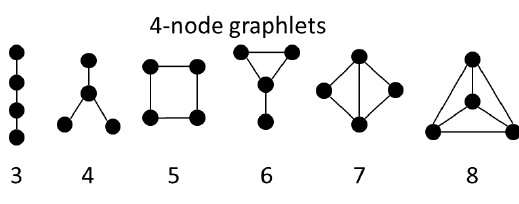
\includegraphics[width=\textwidth]{graphlets.png}
	\caption{Graphlets with 4 nodes}
	\label{fig:graphlets}
\end{marginfigure}
Graphlet kernels enumerate all graph structures of a possible size and count their occurrence in a graph. This is combinatorially difficult and an alternative is to use path-based methods which examine different kinds of paths in the graph. For example, the \textit{random-walk kernel} \cite{random-walk-kernel} involves running random walks all over the graph and then counting the occurrence of different degree sequences, while the \textit{shortest-path kernel} \cite{shortest-path-kernel} uses shortest paths between nodes instead of random-walks.

\subsection{Measures of Neighborhood Overlap}
Now we try to quantify the relation between nodes, which cannot be done using node-level or graph-level kernels. We denote $\mathbf{S} \in \mathbb{R}^{|V| \times |V|}$ as the similarity matrix summarizing the statistics. We commonly take the probability of an edge occurring proportional to the statistical measure, i.e $\mathbb{P}(A_{uv} = 1) \propto \mathbf{S}[u,v]$.
\begin{enumerate}
	\item \textit{Local overlap measures}
\begin{enumerate}
\item \textbf{Common Neighbors (CN)}: It is the simplest neighborhood overlap measure and counts the number of neighbors two nodes share.
\begin{equation}
	\mathbf{S}_{CN}[u, v] = |\mathcal{N}(u) \cap \mathcal{N}(v)|
\end{equation}	
We can extend the idea to local overlap measures defined over CN, denoted by the next three quantifiers.
\item \textbf{Sorensen index}: This normalizes the counts of common neighbours by the sum of node-degrees.
\begin{equation}
	\mathbf{S}_{Sorensen}[u, v] = \dfrac{2|\mathcal{N}(u) \cap \mathcal{N}(v)|}{d_u + d_v}
\end{equation}
\item \textbf{Salton index}: This normalizes using the product of degrees.
\begin{equation}
	\mathbf{S}_{Salton}[u, v] = \dfrac{2|\mathcal{N}(u) \cap \mathcal{N}(v)|}{\sqrt{d_ud_v}}
\end{equation}
\item \textbf{Jaccard index}: This is an IOU measure.
\begin{equation}
	\mathbf{S}_{Jaccard}[u, v] = \dfrac{|\mathcal{N}(u) \cap \mathcal{N}(v)|}{|\mathcal{N}(u) \cup \mathcal{N}(v)|}
\end{equation}
\item \textbf{Resource Allocation (RA)}: It places importance on the common neighbors by summing the inverse degrees, i.e
\begin{equation}
	\mathbf{S}_{RA}[u, v] = \sum_{w \in \mathcal{N}(u) \cap \mathcal{N}(v)} \dfrac{1}{d_w}
\end{equation}
\item \textbf{Adamic-Adar (AA)}: It is similar to RA, just utilizes inverse log of the degrees, i.e
\begin{equation}
	\mathbf{S}_{AA}[u, v] = \sum_{w \in \mathcal{N}(u) \cap \mathcal{N}(v)} \dfrac{1}{\log d_w}
\end{equation}
Both these measures infer that common neighbors with low degrees are more informative.
\end{enumerate}
\item \textit{Global overlap measures}
\begin{enumerate}
	\item \textbf{Katz Index}: We take a discounted count of number of paths of all lengths between a pair of nodes, i.e
	\begin{equation}
		\mathbf{S}_{Katz}[u, v] = \sum_{i=1}^\infty \beta^i A_{uv}^i = \Big((\mathbf{I} - \beta \mathbf{A})^{-1} - \mathbf{I}\Big)[u,v]
	\end{equation}
	Here $\beta \in \mathbb{R}^+$ is our discount, and a small $\beta < 1$ down-weights the importance of long-paths.
\end{enumerate}
\end{enumerate}